\section{Anwendungsfälle und Szenarien}

\subsection{Szenarien}

\subsubsection{Erstausführung}
\paragraph{Erstmaliges Starten der Application}
\begin{itemize}
	\item Der Benutzer startet erstmalig die Application.
	\item Es wird ein Ladebildschirm angezeigt.
	\item Der Benutzer wird automatisch in die Sequenz zur Erstellung eines Profils weitergeleitet. (Siehe Szenario "`Profil anlegen"')
	\item Das soeben angelegte, erste Profil wird automatisch aktiviert und der Benutzer wird ins Hauptmenü des Spiels weitergeleitet.
	\item Durch drücken des Start-Buttons(H1) wird ein erstes Spiel gestartet.
	\item Alternativ stehen dem Benutzer auch alle anderen Funktionen des Hauptmenüs zur Verfügung.
\end{itemize}
\paragraph{Erstes Spiel starten}
\begin{itemize}
	\item Das Spiel überspringt die Levelauswahl und startet gleich mit dem ersten Level (Tutoriallelvel).
	\item Die Hintergrundgeschichte des Spiels wird dem Benutzer innerhalb einer Sequenz erklärt.
	\item Das Spiel startet im Editormodus.
	\item Die wichtigsten Bedienflächen werden schrittweise und nacheinander erklärt (Tutorial).
	\item Das Ziel des Levels wird als Popup angezeigt.
	\item Der Benutzer muss nun zur Erfüllung des Levelziels die im Tutorial erwähnten Buttons und Dialoge benutzen.
	\item Ist dies geschehen, so ist das Tutoriallevel beendet und der Levelabschlussdialog erscheint.
	\item Der Benutzer erhält eine Belohnung und kann nun wahlweise entweder das soeben gespielte Level erneut spielen, zum nächsten Level fortschreiten oder zurück ins Hauptmenü des Spiels gehen.
\end{itemize}

\subsubsection{Level spielen}
\paragraph{Voraussetzungen}
\begin{itemize}
	\item Der Benutzer hat bereits ein Spielerprofil angelegt.
	\item Der Benutzer befindet sich zu Beginn im Hauptmenü.
\end{itemize}
\paragraph{Levelauswahl und -start}
\begin{itemize}
	\item Im Hauptmenü kann der Benutzer sein aktuelles Level (das höchste, noch nicht erfolgreich bestandene Level) durch das Drücken des Start-Buttons(H1) direkt starten.
	\item Alternativ wird der Benutzer durch das Drücken des Level-Buttons(H2) in das Levelauswahlmenü weitergeleitet.
	\item Das Levelauswahlmenü ist als Raster von nummerierten Buttons angeordnet, wobei ein nummerierter Button einem Level entspricht.
	\item Die Höhe der Nummerierung sowie die Farbe des Buttons kennzeichnen den Schwierigkeitsgrad des Levels.
	\item Die Level werden durch drücken des jeweiligen Buttons gestartet.
	\item Ein Level lässt sich erst starten, wenn alle vorherigen Level erfolgreich abgeschlossen wurden.
	\item Am Anfang eines Levels kann es in Folge eines Tutorials zu einer Sequenz kommen, die gegebenenfalls übersprungen werden kann.
	\item Das Levelziel wird als Popup eingeblendet und kann über den Levelziel-Button(G6) im Spiel jederzeit erneut eingesehen werden.
	\item Ein Level startet im Editor-Modus.
\end{itemize}
\paragraph{Editor-Modus}
\begin{itemize}
	\item Nach Anzeigen des Levelziels wird auf dem Bildschirm der aktuelle Zustand des Spielfelds angezeigt.
	\item Zur Ergänzung des Spielfelds und zum Erreichen des Levelziels lassen sich einzelne Spielelemente aus einer Werkzeugleiste per Drag$\&$Drop auf dem Spielfeld platzieren (bei höheren Level).
	\item Beim Platzieren per Drag$\&$Drop werden Platzierungflächen als Hilfe zur geeigneten Absetzung der Elemente hervorgehoben.
	\item Beim Drücken auf ein Spielelement (Lamm oder Edelstein) öffnet sich ein Farbauswahldialog mit acht Farben.
	\item Nachdem der Benutzer ein Farbe ausgewählt hat, färbt sich das entsprechende Spielelement in dieser Farbe und der Farbauswahl-Dialog schließt sich.
	\item Zum Entfernen von Spielelementen aus dem Spielfeld können die jeweiligen Spielelemente ebenfalls per Drag$\&$Drop in die Werkzeugleiste zurückgelegt werden.
	\item Durch das Drücken des Hinweis-Buttons(G2) wird dem Benutzer ein Lösungsansatz zum erreichen des Levelziels als Popup angezeigt.
	\item Durch des Drücken des Pause-Buttons(G1) wird das Pausenmenü aufgerufen.
	\item Im Pausenmenü lässt sich das Level durch das Drücken des jeweiligen Buttons wahlweise entweder fortsetzen oder in seinen Anfangszustand zurücksetzen oder es kann zum Hauptmenü zurückgekehrt werden.
	\item Der Reduktions-Modus ist über den Reduktions-Button(G5) erreichbar. 
	\item Es lässt sich erst zum Reduktions-Modus wechseln, wenn alle Spielelemente auf dem Spielfeld eingefärbt sind.
\end{itemize}

\paragraph{Reduktion-Modus}
\begin{itemize}
	\item Der Benutzer befindet sich nun im Reduktions-Modus.
	\item Das Spielfeld befindet sich in dem Zustand, der im Editor-Modus erstellt wurde.
	\item Gemäß den Spielregeln wird die Anordnung von Spielelementen auf dem Spielfeld reduziert.
	\item Alle Reduktionsschritte werden auf dem Spielfeld dargestellt.
	\item Es ist wahlweise eine vollständige, automatische Reduktion oder eine schrittweise Reduktion möglich.
	\item Die automatische Reduktion wird vom Benutzer durch das Drücken des Abspiel-Buttons(R2), der auch zur Pausierung der Reduktion genutzt wird, gesteuert.
	\item Die schrittweise Reduktion wird vom Benutzer durch das Drücken des Schritt-Vorwärts-Buttons(R1) und des Schritt-Rückwärts-Buttons(R3) gesteuert.
	\item Der Vorgang läuft solang bis gemäß der gewählten Reduktionsstrategie die Anordnung nicht mehr weiter reduziert werden kann.
	\item Dann wird überprüft, ob das Levelziel erreicht wurde.
	\item Anschließend erscheint der Levelabschlussdialog, der den Benutzer darüber informiert, ob dieser das Level erfolgreich abgeschlossen hat oder nicht.
	\item Beim erstmaligen erfolgreichen Bestehen des Levels erhält der Benutzer eine Belohnung, die im Levelabschlussdialog ebenfalls angezeigt wird.
	\item Nun kann der Benutzer noch wahlweise durch das Drücken des jeweiligen Buttons das soeben gespielte Level erneut spielen, zum nächsten Level fortschreiten (nur bei einem erfolgreichen Abschluss des Levels) oder zurück ins Hauptmenü des Spiels gehen.
\end{itemize}

\subsubsection{Profil anlegen}
\paragraph{Voraussetzungen}
\begin{itemize}
	\item Der Benutzer befindet sich im Szenario "`Erstausführung"' oder er drückt auf den Hinzufügen-Button(P3) des Profilauswahlmenüs oder er drückt auf den Konfigurations-Button(P2) neben einem vorhanden Profil im Profilauswahlmenü.
\end{itemize}
\paragraph{Profilanlegung}
\begin{itemize}
	\item Der Benutzer wählt zunächst im Sprachauswahlmenü seine Sprache.
	\item Die voreingestellte Sprache lässt sich über die Pfeil-Buttons(S2) ändern.
	\item Über den Weiter-Button(B1) gelangt der Benutzer zum nächsten Dialogfenster,dem Namenswahlmenü.
	\item Durch das Drücken auf die Namenseingabe-Textbox(N1) öffnet sich die Eingabemethode.
	\item Der Benutzer gibt seinen Namen ein.
	\item Falls das Textbox noch leer ist oder falls der Name bereits für ein anderes Profil vorhanden ist, so bleibt der Weiter-Button deaktiviert.
	\item Bei gültiger Eingabe eines Namens kann der Benutzer zum Avatarauswahlmenü wechseln.
	\item In diesem Dialogfenster kann der Benutzer aus einer vorgegebenen Auswahl von Avatarbildern mittels Pfeil-Buttons(A2) wählen.
	\item Mittels der einzelnen Zurück- und Weiter-Button können nochmals die Einstellungen des Profils bearbeitet werden oder das Profil kann durch das Drücken des Bestätigungsbuttons (TODO) fertig gestellt werden.
	\item Dem Benutzer erscheint nun automatisch ein Popup zur Begrüßung, auf dem sein Profilname und sein gewähltes Avatarbild angezeigt wird.
\end{itemize}

\subsubsection{Profilverwaltung}
\paragraph{Voraussetzungen}
\begin{itemize}
	\item Der Benutzer besitzt ein Spielerprofil.
	\item Der Benutzer befindet sich zu Beginn im Hauptmenü.
\end{itemize}
\paragraph{Neues Profil anlegen}
\begin{itemize}
	\item Der Benutzer drückt im Hauptmenü auf den Logout-Button(H7), wodurch er sich mit seinem aktuellen Profil automatisch abmeldet und in das das Profilauswahlmenü weitergeleitet wird.
	\item Im Profilauswahlmenü werden alle bereits erstellte Profile mit Namen und Avatar angezeigt.
	\item Der Benutzer drückt im Profilauswahlmenü auf den Button zum Hinzufügen von neuen Profilen.
	\item Der Benutzer wird nun zur Profilanlegungs-Sequenz des Szenarios "`Profil anlegen"' weitergeleitet.
	\item Anschließend befindet sich der Benutzer mit seinem neuen Profil wieder im Hauptmenü.
\end{itemize}
\paragraph{Profil bearbeiten }
\begin{itemize}
	\item Der Benutzer drückt im Profilauswahlmenü den Konfigurationsbutton(P2) neben dem entsprechenden Profil, das er bearbeiten will, wodurch ein Dialog zur Entscheidung zwischen Profilbearbeitung und dem Löschen des Profils geöffnet wird.
	\item Falls nur ein Spielerprofil existiert, fehlt die Option zum Löschen des Profils im Dialogfenster.
	\item Der Benutzer drückt nun im Dialogfenster auf die Option zur Bearbeitung des Profils. 
	\item Der Benutzer wird nun zur Profilanlegungs-Sequenz des Szenarios "`Profil anlegen"' weitergeleitet (die bisherigen Einstellungen des Profils sind als Voreinstellungen gesetzt).
	\item Anschließend befindet sich der Benutzer wieder im Profilauswahlmenü.1
\end{itemize}

\subsubsection{Profil wechseln}
\paragraph{Voraussetzungen}
\begin{itemize}
	\item Es sind bereits mindestens zwei Profile angelegt worden.
	\item Der Benutzer befindet sich zu Beginn im Profilauswahlmenü.
\end{itemize}
\paragraph{Profil wechseln}
\begin{itemize}
	\item Der Benutzer drückt im Profilauswahlmenü auf das Profil, auf das er wechseln will(Name-Button, P1).
	\item Der Benutzer wird automatisch mit seinem neuen Profil, welches nun aktiviert ist, zum Hauptmenü weitergeleitet.
\end{itemize}

\subsubsection{Profil löschen}
\paragraph{Voraussetzungen}
\begin{itemize}
	\item Es sind bereits mindestens zwei Profile angelegt worden.
	\item Der Benutzer befindet sich zu Beginn im Profilauswahlmenü.
\end{itemize}
\paragraph{Profil löschen}
\begin{itemize}
	\item Der Benutzer drückt im Profilauswahlmenü den Konfigurationsbutton(P2) neben dem entsprechenden Profil, das er bearbeiten will, wodurch ein Dialog zur Entscheidung zwischen Profilbearbeitung und dem Löschen des Profils geöffnet wird.
	\item Der Benutzer drückt die Option zum Löschen des Profils.
	\item Es erscheint ein Dialogfenster, in dem der Benutzer gefragt wird, ob er sich sicher ist, dass er dieses Profil löschen will.
	\item Verneint der Benutzer die Frage, dann bricht der Löschvorgang ab und der Benutzer befindet sich wieder im normalen Profilauswahlmenü.
	\item Falls der Benutzer den Vorgang bestätigt, erscheint ein Popup, das die Bestätigung des Löschvorgangs und das gelöschte Profil anzeigt.
	\item Der Benutzer wird nun automatisch zum aktualisierten Profilauswahlmenü weitergeleitet, in dessen Profilliste das soeben gelöschte Profil entfernt wurde.
\end{itemize}

\subsubsection{Einstellungen ändern}
\paragraph{Voraussetzungen}
\begin{itemize}
	\item Der Benutzer befindet sich zu Beginn im Hauptmenü.
\end{itemize}
\paragraph{Einstellungen ändern}
\begin{itemize}
	\item Der Benutzer drückt im Hauptmenü auf den Optionen-Button(H4), was ihn zum Optionenmenü weiterleitet.
	\item Im Optionenmenü befinden sich
	\begin{itemize}
		\item Die Lehrermodus-Checkbox(O1)
		\item Die Farbenblindenmodus-Checkbox(O2)
		\item Der Statistik-Button(O3) zum Anzeigen der Statistik.
		\item Ein Geräusche-Slider(O4)
		\item Ein Musik-Slider(O5)
	\end{itemize}
	\item Der Benutzer kann alle Einstellungen ändern bis er zufrieden mit ihnen ist.
	\item Die der Geräusche-Slider gibt beim loslassen des Sliders ein Testgeräusch von sich.
	\item Die Geräusche- und Musikeinstellungen sind relativ zur eigentlichen Medienlautstärke.
	\item Alle Änderungen an den Einstellungen werden sofort übernommen und für das aktuelle, aktivierte Profil gespeichert.
	\item Durch das Drücken des Hilfsbutton erhält der Benutzer mehr Informationen zu den Einstellungsoptionen.
	\item Durch das Drücken des Zurück-Buttons gelangt der Benutzer zurück in das Hauptmenü.
\end{itemize}

\subsubsection{Münzen gegen Belohnungen eintauschen}
\paragraph{Voraussetzungen}
\begin{itemize}
	\item Es existiert mindestens ein Spielerprofil.
	\item Der Benutzer befindet sich zu Beginn im Hauptmenü.
\end{itemize}
\paragraph{Belohnungen eintauschen}
\begin{itemize}
	\item Der Benutzer drückt im Hauptmenü auf den Einkaufs-Button(H6), auf dem sein aktueller Münustand angezeigt wird, wodurch das Einkaufsmenü geöffnet wird.
	\item Die Belohnungen sind im Einkaufsmenü in die Kategorien Musik, Hintergründe (für Level) und Texturen eingeteilt.
	\item Die Belohnungen werden durch das Bezahlen mit Münzen (die übliche Belohnung für das erstmalige bestehen eines Levels) gekauft und danach nach Belieben aktiviert.
	\item Es gibt pro Kategorie ein Dropdownmenü.
	\item Beim Drücken des Dropdownmenüs wird eine Liste mit den einzelnen Belohnungen der Kategorie aufgeklappt.
	\item Beim erneuten Drücken des selben Dropdownmenüs wird die Kategorieliste wieder zugeklappt.
	\item Pro Belohnung in der Kategorieliste sind der Belohnungsname, die Kosten in Münzen sowie eine Checkbox für die mögliche Aktivierung nach einem Kauf aufgelistet.
	\item Falls der Benutzer nun eine Belohnung aus der Musik-Kategorie will, muss er zunächst auf das Musik-Dropdownmenü drücken.
	\item In nun aufklappenden Musik-Dropdownmenü wählt er eine Belohnung aus, für die er genügend Münzen besitzt.
	\item Nun öffnet sich ein Dialogfenster zur Bestätigung des Kaufs.
	\item Falls der Benutzer den Kaufvorgang bestätigt, wird die Bestätigung des Vorgangs in einem Popup angezeigt, falls nicht so wird der Kaufvorgang abgebrochen.
	\item Der neue Münzenstand wird nun im Einkaufsmenü angezeigt.
	\item Bereits gekaufte Belohnungen werden im Einkaufsmenü hervorgehoben.
	\item Belohnungen, die aufgrund des aktuellen Münzstandes nicht erworben werden können, werden nicht in einer Kategorieliste aufgelistet.
	\item Manche erworbene Belohnungen können nicht zur selben Zeit in einem Profil aktiviert sein, wie beispielsweise die Belohnungen der Musik-Kategorie.
	\item Durch das Drücken des Zurück-Buttons(B2) des Einkaufsmenüs kehrt der Benutzer wieder ins Hauptmenü zurück.
\end{itemize}

\subsubsection{Erfolgsansicht}
\paragraph{Voraussetzungen}
\begin{itemize}
	\item Es existiert mindestens ein Spielerprofil.
	\item Der Benutzer befindet sich zu Beginn im Hauptmenü.
\end{itemize}
\paragraph{Erfolge ansehen}
\begin{itemize}
	\item Der Benutzer drückt den Erfolge-Button(H3) im Hauptmenü, wodurch das Erfolgsmenümenü geöffnet wird.
	\item Die Erfolge sind im ERfolgsmenü in Kategorien eingeordnet.
	\item Jeder Erfolg wird als ein Label dargestellt.
	\item Bereits vom Spielerprofil freigeschaltete Erfolge sind hervorgehoben und aktiviert, noch nicht freigeschaltete Erfolge sind deaktiviert.
	\item Durch das Drücken des Zurück-Buttons(B2) kehrt der Benutzer ins Hauptmenü zurück.
\end{itemize}

% \subsubsection{Level erzeugen im freien Modus} , es fehlt noch ein Button dafür in der GUI

\subsubsection{Betriebssysteminteraktion}
\begin{itemize}
	\item Der Benutzer befindet sich während des Spielens eines Levels in einem Spielmodus (Editor-Modus, Reduktion-Modus oder Freier Modus)
	\item Es kann nötig werden, das Spiel direkt ohne Umwege über Menüs zu verlassen.
	\item Dies kann bspw. bei der Betätigung des "`Home"'-Buttons  oder auch bei Betriebssystemereignissen geschehen.
	\item Die Application soll in diesem Fall den aktuellen Zustand, also die Anordnung der Spielelemente auf dem Spielfeld, abspeichern.
	\item Beim Neustart der Application soll es so möglich sein, die vorherige Konstellation der Spielelemente wiederherzustellen.
\end{itemize}

\subsection{Anwendungsfälle}

\begin{figure}[H]
\centering
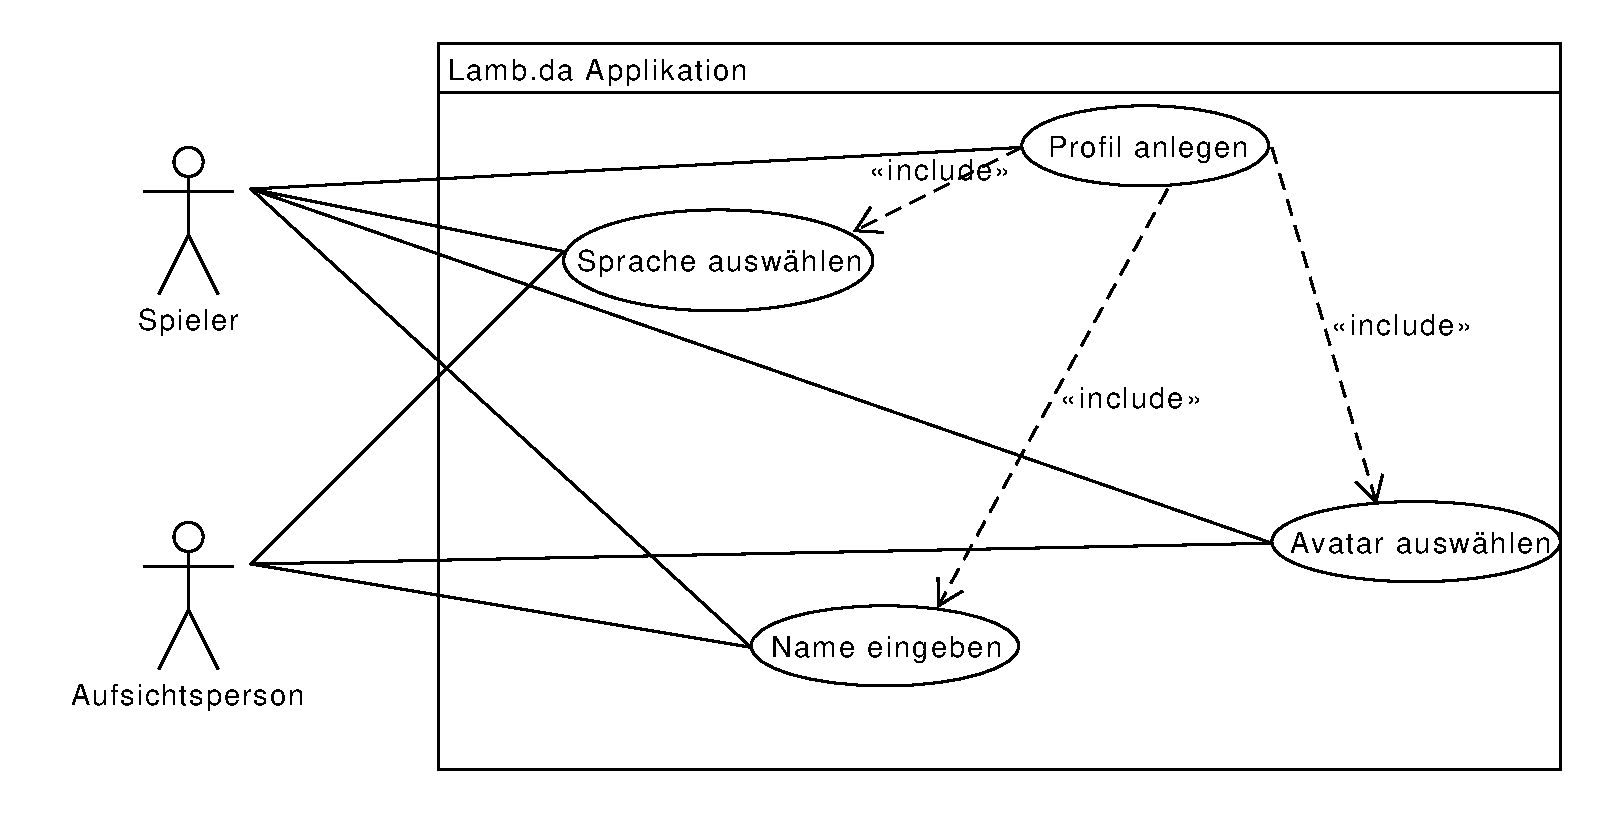
\includegraphics[scale=0.55]{../use_cases/create_profile.pdf}
\caption{Anwendungsfalldiagramm Profil Anlegen}
\end{figure}

\begin{figure}[H]
\centering
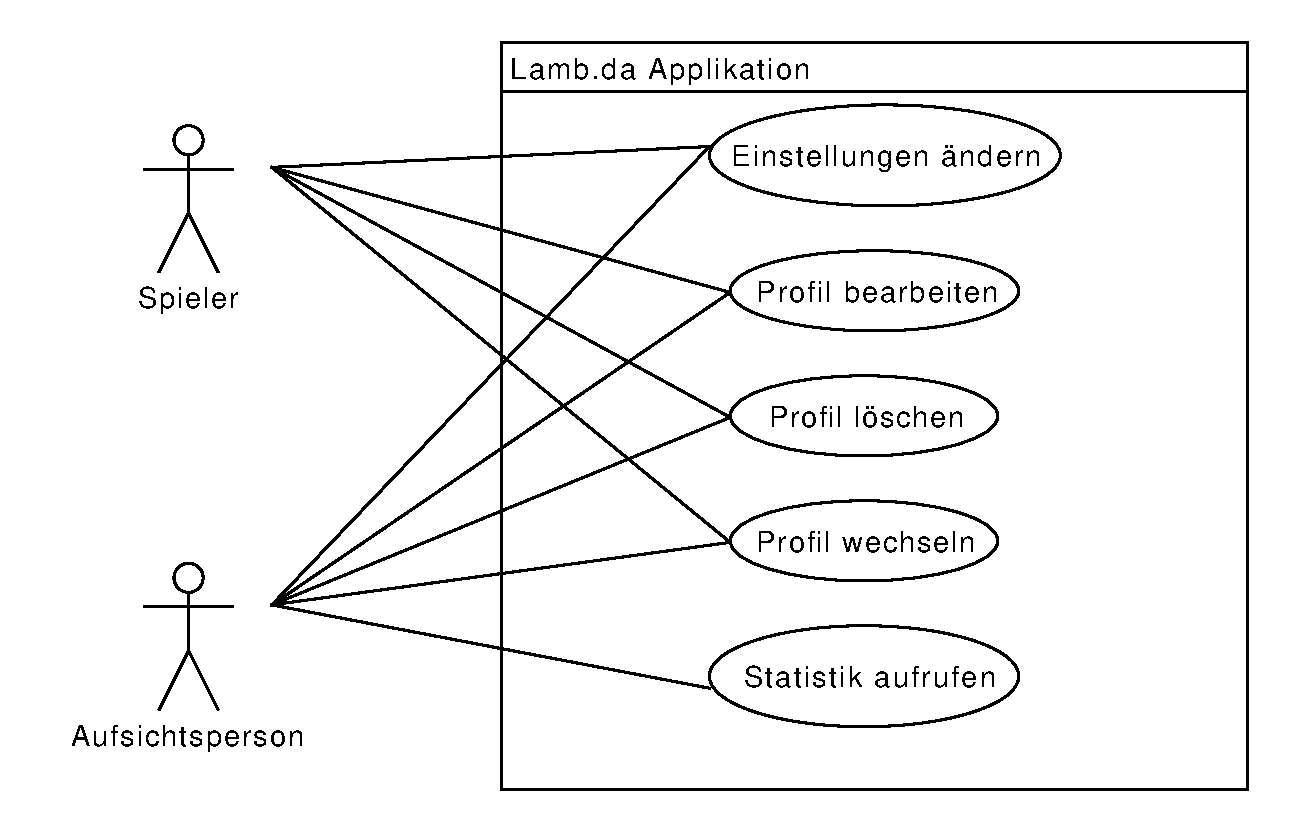
\includegraphics[scale=0.55]{../use_cases/game_settings.pdf}
\caption{Anwendungsfalldiagramm Spieleinstellungen}
\end{figure}

\begin{figure}[H]
\centering
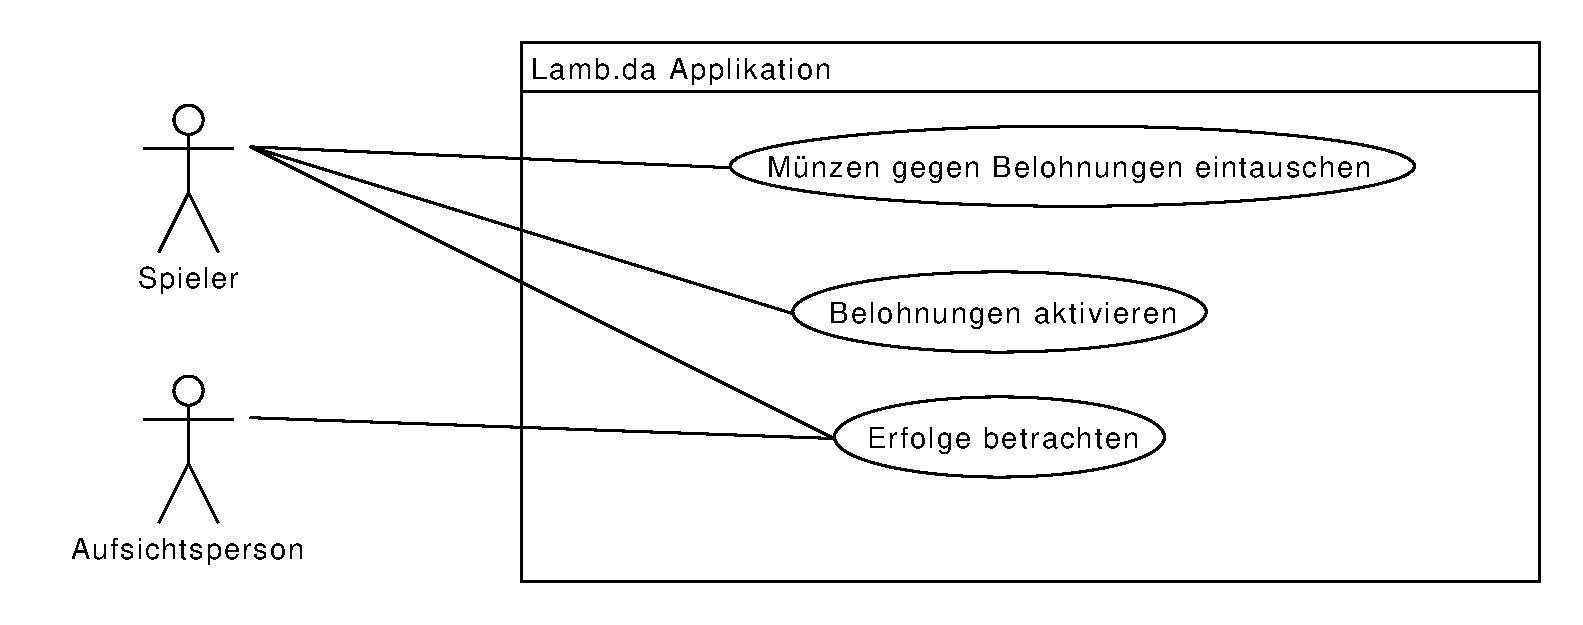
\includegraphics[scale=0.55]{../use_cases/gamification.pdf}
\caption{Anwendungsfalldiagramm Gamification}
\end{figure}

\begin{figure}[H]
\centering
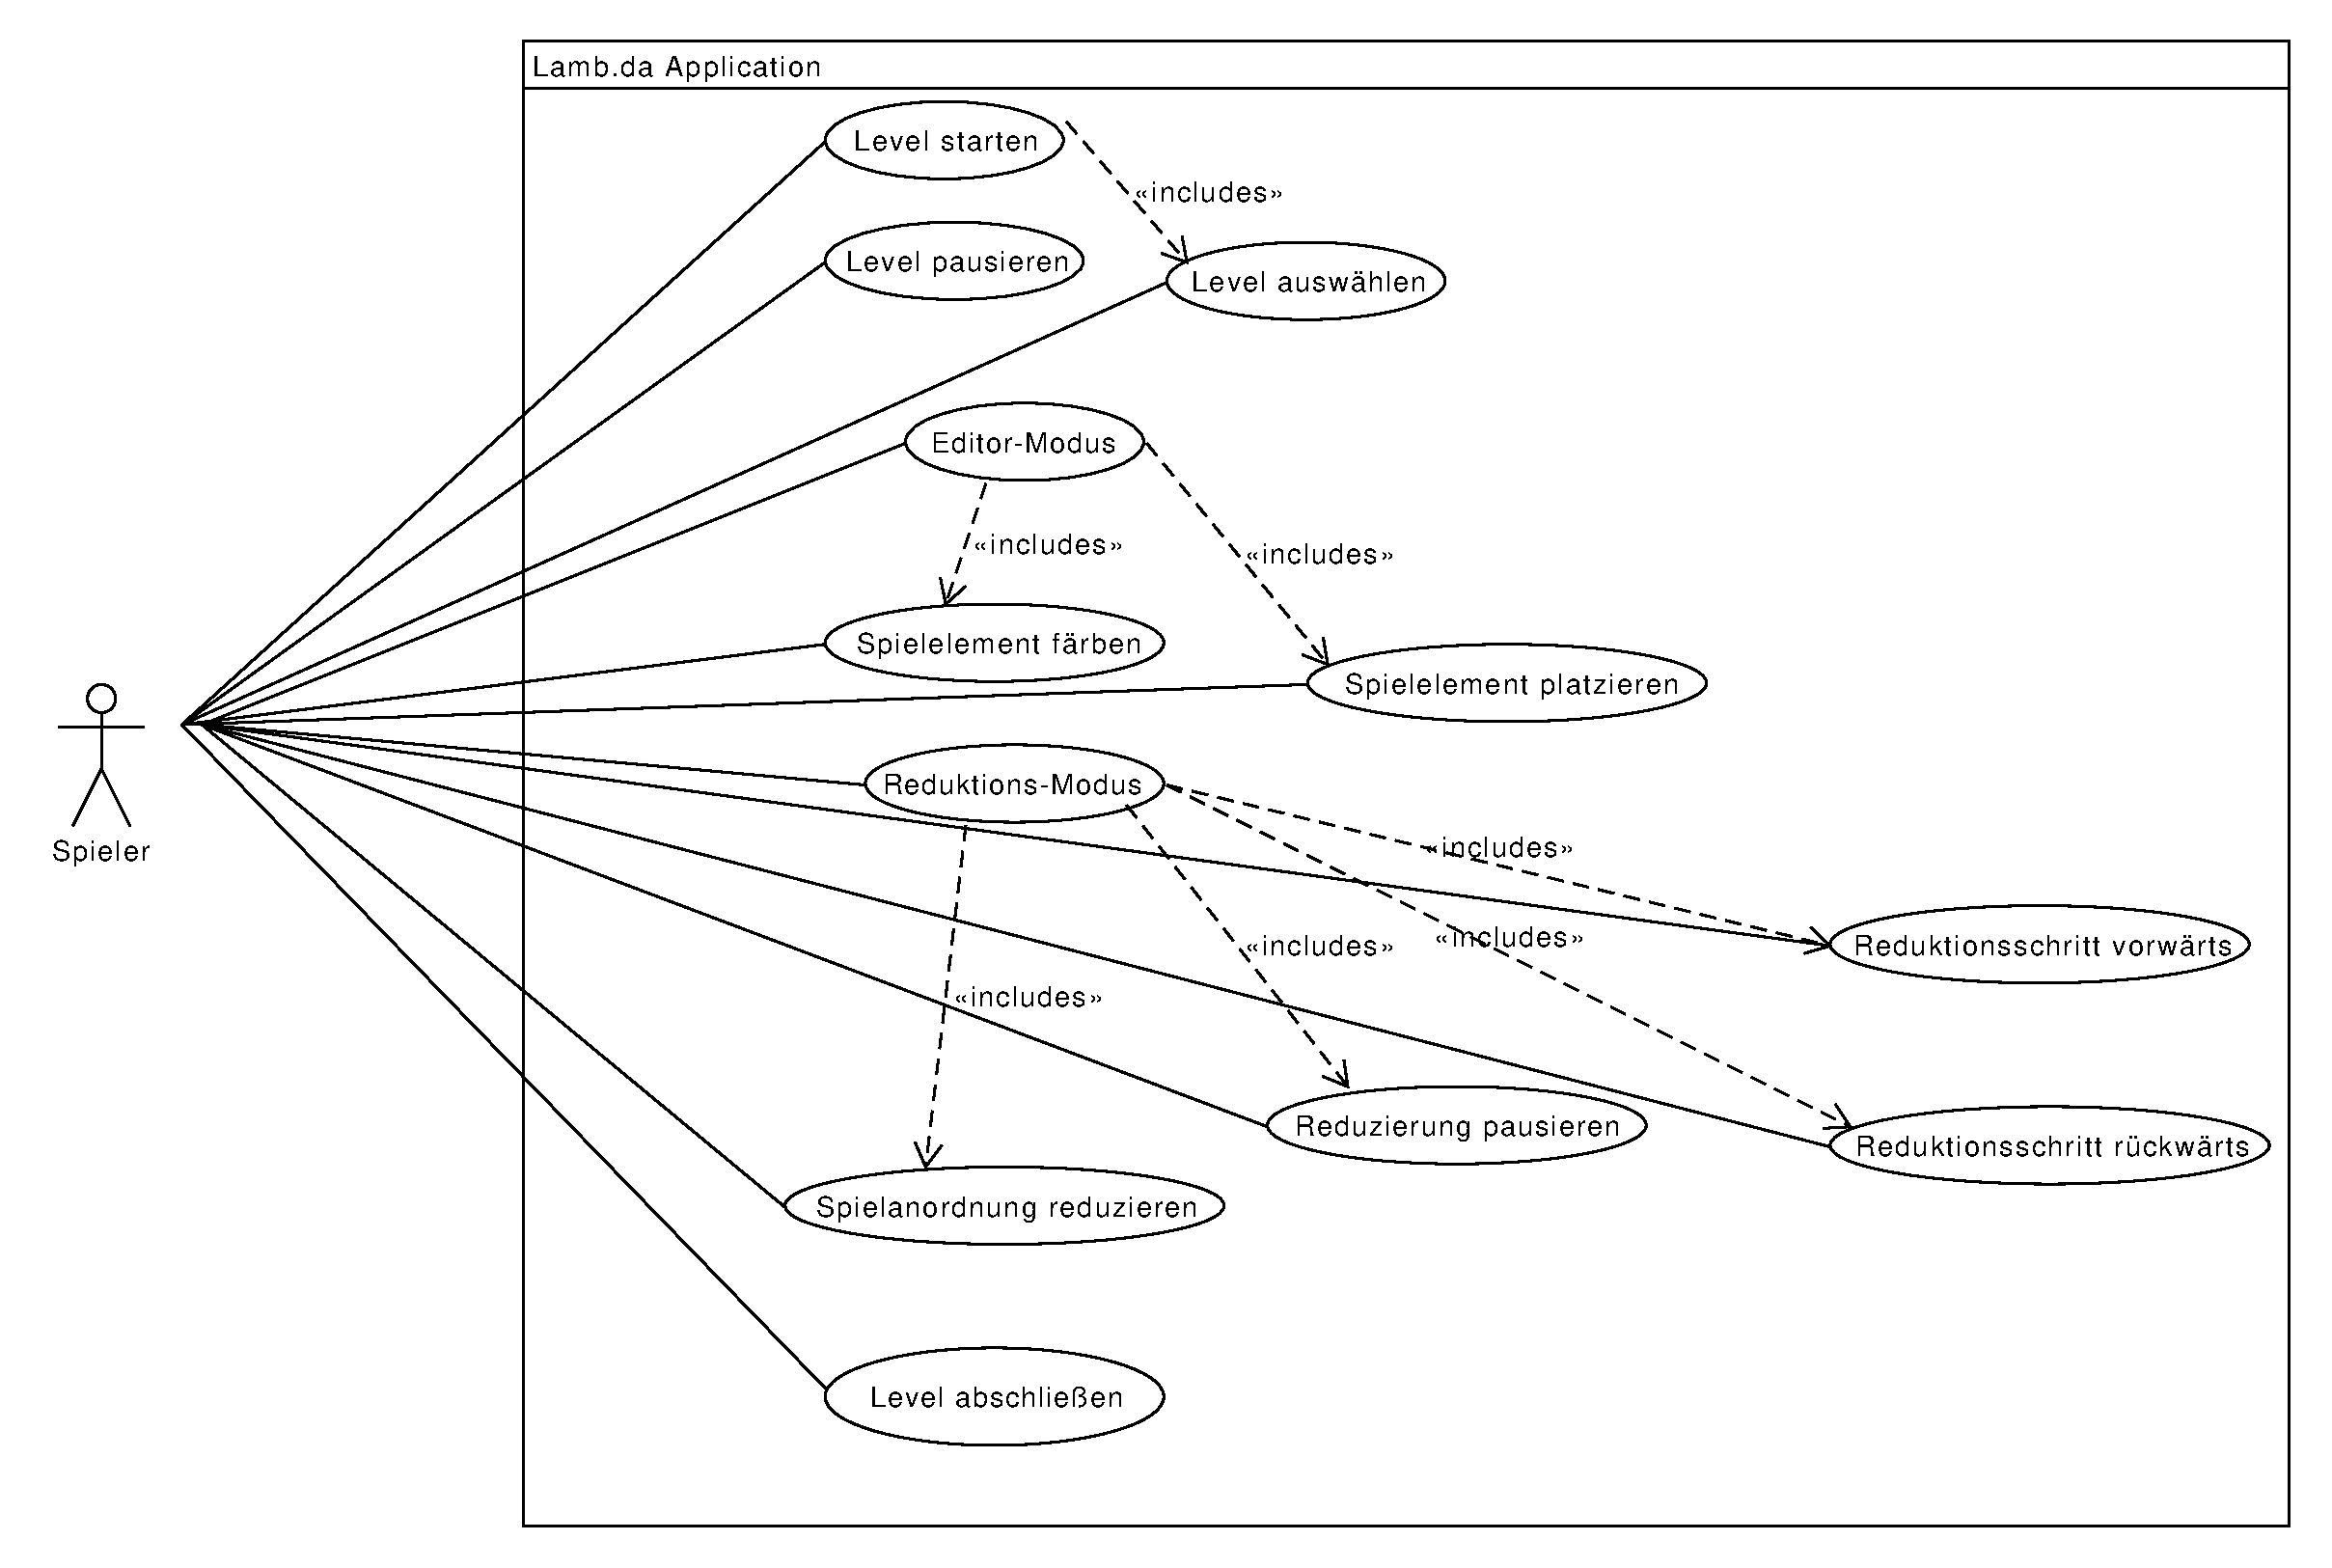
\includegraphics[scale=0.40]{../use_cases/play_level.pdf}
\caption{Anwendungsfalldiagramm Level Spielen}
\end{figure}